%File: anonymous-submission-latex-2023.tex
\documentclass[letterpaper]{article} % DO NOT CHANGE THIS
\usepackage{aaai23}  % DO NOT CHANGE THIS
\usepackage{times}  % DO NOT CHANGE THIS
\usepackage{helvet}  % DO NOT CHANGE THIS
\usepackage{courier}  % DO NOT CHANGE THIS
\usepackage[hyphens]{url}  % DO NOT CHANGE THIS
\usepackage{graphicx} % DO NOT CHANGE THIS
\urlstyle{rm} % DO NOT CHANGE THIS
\def\UrlFont{\rm}  % DO NOT CHANGE THIS
\usepackage{natbib}  % DO NOT CHANGE THIS AND DO NOT ADD ANY OPTIONS TO IT
\usepackage{caption} % DO NOT CHANGE THIS AND DO NOT ADD ANY OPTIONS TO IT

\frenchspacing  % DO NOT CHANGE THIS
\setlength{\pdfpagewidth}{8.5in} % DO NOT CHANGE THIS
\setlength{\pdfpageheight}{11in} % DO NOT CHANGE THIS
%
% These are recommended to typeset algorithms but not required. See the subsubsection on algorithms. Remove them if you don't have algorithms in your paper.
\usepackage{algorithm}
\usepackage{algorithmic}


%%%%% ADDED PACKAGES

\usepackage{subcaption}
\usepackage{paralist}
%
% These are are recommended to typeset listings but not required. See the subsubsection on listing. Remove this block if you don't have listings in your paper.
\usepackage{newfloat}
\usepackage{listings}
\DeclareCaptionStyle{ruled}{labelfont=normalfont,labelsep=colon,strut=off} % DO NOT CHANGE THIS
\lstset{%
	basicstyle={\footnotesize\ttfamily},% footnotesize acceptable for monospace
	numbers=left,numberstyle=\footnotesize,xleftmargin=2em,% show line numbers, remove this entire line if you don't want the numbers.
	aboveskip=0pt,belowskip=0pt,%
	showstringspaces=false,tabsize=2,breaklines=true}
\floatstyle{ruled}
\newfloat{listing}{tb}{lst}{}
\floatname{listing}{Listing}
%
% Keep the \pdfinfo as shown here. There's no need
% for you to add the /Title and /Author tags.
\pdfinfo{
/TemplateVersion (2023.1)
}

% DISALLOWED PACKAGES
% \usepackage{authblk} -- This package is specifically forbidden
% \usepackage{balance} -- This package is specifically forbidden
% \usepackage{color (if used in text)
% \usepackage{CJK} -- This package is specifically forbidden
% \usepackage{float} -- This package is specifically forbidden
% \usepackage{flushend} -- This package is specifically forbidden
% \usepackage{fontenc} -- This package is specifically forbidden
% \usepackage{fullpage} -- This package is specifically forbidden
% \usepackage{geometry} -- This package is specifically forbidden
% \usepackage{grffile} -- This package is specifically forbidden
% \usepackage{hyperref} -- This package is specifically forbidden
% \usepackage{navigator} -- This package is specifically forbidden
% (or any other package that embeds links such as navigator or hyperref)
% \indentfirst} -- This package is specifically forbidden
% \layout} -- This package is specifically forbidden
% \multicol} -- This package is specifically forbidden
% \nameref} -- This package is specifically forbidden
% \usepackage{savetrees} -- This package is specifically forbidden
% \usepackage{setspace} -- This package is specifically forbidden
% \usepackage{stfloats} -- This package is specifically forbidden
% \usepackage{tabu} -- This package is specifically forbidden
% \usepackage{titlesec} -- This package is specifically forbidden
% \usepackage{tocbibind} -- This package is specifically forbidden
% \usepackage{ulem} -- This package is specifically forbidden
% \usepackage{wrapfig} -- This package is specifically forbidden
% DISALLOWED COMMANDS
% \nocopyright -- Your paper will not be published if you use this command
% \addtolength -- This command may not be used
% \balance -- This command may not be used
% \baselinestretch -- Your paper will not be published if you use this command
% \clearpage -- No page breaks of any kind may be used for the final version of your paper
% \columnsep -- This command may not be used
% \newpage -- No page breaks of any kind may be used for the final version of your paper
% \pagebreak -- No page breaks of any kind may be used for the final version of your paper
% \pagestyle -- This command may not be used
% \tiny -- This is not an acceptable font size.
% \vspace{- -- No negative value may be used in proximity of a caption, figure, table, section, subsection, subsubsection, or reference
% \vskip{- -- No negative value may be used to alter spacing above or below a caption, figure, table, section, subsection, subsubsection, or reference

\setcounter{secnumdepth}{0} %May be changed to 1 or 2 if section numbers are desired.

% The file aaai23.sty is the style file for AAAI Press
% proceedings, working notes, and technical reports.
%

% Title

% Your title must be in mixed case, not sentence case.
% That means all verbs (including short verbs like be, is, using, and go),
% nouns, adverbs, and adjectives should be capitalized, including both words in hyphenated terms, while
% articles, conjunctions, and prepositions are lower case unless they
% directly follow a colon or long dash

\title{Sudoku Assistant - An AI-powered app to help solve pen-and-paper Sudokus}
\author{
    %Authors
    % All authors must be in the same font size and format.
    Tias Guns\textsuperscript{\rm1, \rm 2},   
    Emilio Gamba\textsuperscript{\rm1, \rm 2},
    Maxime Mulamba\textsuperscript{\rm1, \rm 2},
    Ignace Bleukx\textsuperscript{\rm 2},
    Senne Berden\textsuperscript{\rm 2},
    Milan Pesa\textsuperscript{\rm 2},
}
\affiliations{
    %Afiliations
    \textsuperscript{\rm 1}Vrije Universiteit Brussel, 
%    Pleinlaan 2, 1050 Brussels, Belgium \\
%    \{emilio.gamba, maxime.mulamba\}@vub.be,\\
\{firstname.lastname@vub.be\} \\
    \textsuperscript{\rm 2}KU Leuven, 
%    Oude Markt 13, 3000 Leuven, Belgium \\
    % email address must be in roman text type, not monospace or sans serif
%    \textsuperscript{\rm 1} firstname.lastname@vub.be, 
%\{tias.guns, ignace.bleuckx, senne.berden, milan.pesa\}@kuleuven.be %\\
\{firstname.lastname\}@kuleuven.be \\
    %\textsuperscript{\rm 3}
%
% See more examples next
}


\begin{document}

\maketitle


\begin{abstract}
The Sudoku Assistant app is an AI assistant that combines machine learning and constraint programming techniques, to interpret and explain a pen-and-paper Sudoku scanned with a smartphone.
Although the demo is about Sudoku, the underlying techniques are equally applicable to other constraint solving problems like timetabling, scheduling, and vehicle routing.
\end{abstract}
%
%\begin{itemize}
%	\item 2-page short paper describing their system
%	\item  1 page of references only
%	\item a video (of duration up to 10 minutes) of the proposed demonstration (Slides are also permitted in lieu of video, but greater weight will be given to submissions accompanied by videos)
%\end{itemize}
%
%\section{Introduction}
%
%
%
%Installation instructions: search for “Sudoku Assistant” on the google play store and verify that the logo matches the above.
%WARNING: at the time this document is written, the app is still under review by Google. It may take a few more days to be available on the play store…
%
%Workings and role of CP:
%The app uses a combination of machine learning and constraint programming techniques to:
%1) use a neural network to estimate the digit written in each square
%2) use constraint programming to verify that the digit estimates make up a valid sudoku, and if not search for an interpretation that does
%
%Use the app to take a picture of a pen-and-paper sudoku. It can contain both printed and hand-written digits. The app will analyze the image and split it into 81 cells, and for each of them, a prediction will be made using an SVHN-trained neural network. The app visualizes the probabilities of each possible value (numbers 1-9 or an empty cell).
%
%Any neural network can make errors, due to the quality of the image or the network itself. So we use constraint programming techniques to find the combination of predictions that leads to a valid, unique sudoku. In this way, constraint reasoning can correct some of the errors that the network makes. With the same technique, it will also correct mistakes that you may have made during solving!
%
%This constraint-based reasoning happens when the app shows 'solving sudoku'. For efficiency reasons, it only considers the most likely predictions of each cell, so you might see "No Sudoku's Found". Usually, this happens when the grid was insufficiently well aligned when taking the picture (we are working on improving this).
%
%Future work: we are working on a ‘Hint’ button that will show what the easiest next move is, based on computing the smallest explanation for every undiscovered value. This uses a constraint solver to find a Minimal Unsatisfiable Subset for (the negation of) each of these values. This explanation technology is expected to be integrated into the app by the end of July.
%We also plan to improve the visual appeal and the usage speed of the app once the above functionality is completed.
%
%
%\section{System design}
%
%
%\section{Visual solving}
%\paragraph{Detecting the Sudoku grid}
%\begin{itemize}
%	\item using a technique for recognizing the sudoku grid and splitting the images
%\item Improvements on current model
%\begin{itemize}
%	\item Stabilize the image 
%	\item Auto take a picture as soon as you find a sudoku grid
%\end{itemize}
%\end{itemize}
%
%\paragraph{Identifying Sudoku numbers}
%% \subsection{Integrating constraint solving in computer vision}
%\begin{itemize}
%    \item \textbf{Visual sudoku}: explaining how the constraint solving can be linked to the computer vision probabilities to select a grid that is satisfiable according to the sudoku constraints
%    	\item Improvements on current models
%    \begin{itemize}
%    \item Scan a faulty Sudoku and get an explanation to debug
%    \item 
%    \end{itemize}
%\end{itemize}
%
%\section{Explanations during solving}
%
%\paragraph{Solving Preferences}
%
%\paragraph{Explaining human-errors} When solving a Sudoku puzzle, a user might be faced with a contradiction. For instance, same numbers appear in the same column, row, or block. This situation is the direct consequence of an error in the puzzle solving process. 
%To help a user debug the inconsistency, we rely on the extraction of a Minimal Unsatisfiable Subset (MUS)\cite{muses}. A smallest MUS will correspond to the \emph{smallest} explanation of unsatisfiability\cite{smus}. In the Sudoku case we consider, the problem constraints are weighted to emulate user preferences, which requires extraction of an \textit{optimal} (minimal weight) unsatisfiable subset \cite{ocus}.
%
%\paragraph{Providing preferred hints}
%
%\section{Demonstration}
%%% Something about the way the demonstration is going to be used by the public
%



%The demo uses recently published hybrid classification and reasoning for image-based constraint solving techniques.\cite{MAXIMEsPaper} It uses a convolutional neural network to recognize what is in each of the 81 cells, including printed and handwritten digits. 
%More specifically it predicts the probablility that it is empty or numbers 1-9, including hand-written ones. 
%Errors of the network (or the user) are corrected by using a constraint solver to validate that the predictions make up a valid Sudoku. If not, the solver computes the most likely prediction combination that is valid.

%Furthermore, the demo also shows recently published techniques for step-wise explanations of constraint satisfaction problems. The result is a hint mechanism highlights which existing digits and constraints can be used to derive that new value. It will compute the provably cheapest explanation over all empty cells. While the app does this in a generic way, without knowing the tricks of the game, the visualisations provided are rich enough for users to learn new tricks along the way.
%\section{Introduction}


%Nowadays, pen-and-paper puzzles are very popular, ranging from blogs featuring a wide range of strategies to solve Sudoku puzzles to video tutorials on how to solve the most-difficult Sudoku.
%
%Something something about being stuck solving and have a quick hint about what to do next



\section{System overview}

The Sudoku Assistant is a smartphone app that features two components:
\begin{inparaenum}[(1)]
	\item a \emph{hybrid predict-and-reasoning system} to recognize the digits of a Sudoku grid from a picture taken by a smartphone camera; and
	\item a \emph{hinting mechanism} to guide the user into finding the solution.
\end{inparaenum}

\subsection{Phase 1: Hybrid of prediction and reasoning}
The predict-and-reasoning component uses a classifier to recognize the digits in the Sudoku grid as well as a reasoning engine in order to solve the Sudoku puzzle. 
%The app combines the classification task with the reasoning aspect to correct wrongly predicted digits into a hybrid predict-and-reasoning.

%\paragraph{Predicting the digits}
\paragraph{Recognizing the Sudoku digits}

First, the Sudoku Assistant app invites the user to align the overlay with the Sudoku grid (see Fig. \ref{fig:camera}). 
After a picture of a Sudoku puzzle is taken with the app, the picture is segmented into 81 cells. 
 A pre-trained convolutional neural network (CNN) is then applied to each cell in order to make a digit prediction. For each cell, the output of the CNN is a probability distribution over the 10 possible values: digits 1-9 and the empty cell value. 

\begin{figure}[!h]
	\begin{subfigure}{0.15\textwidth}
		\centering
%		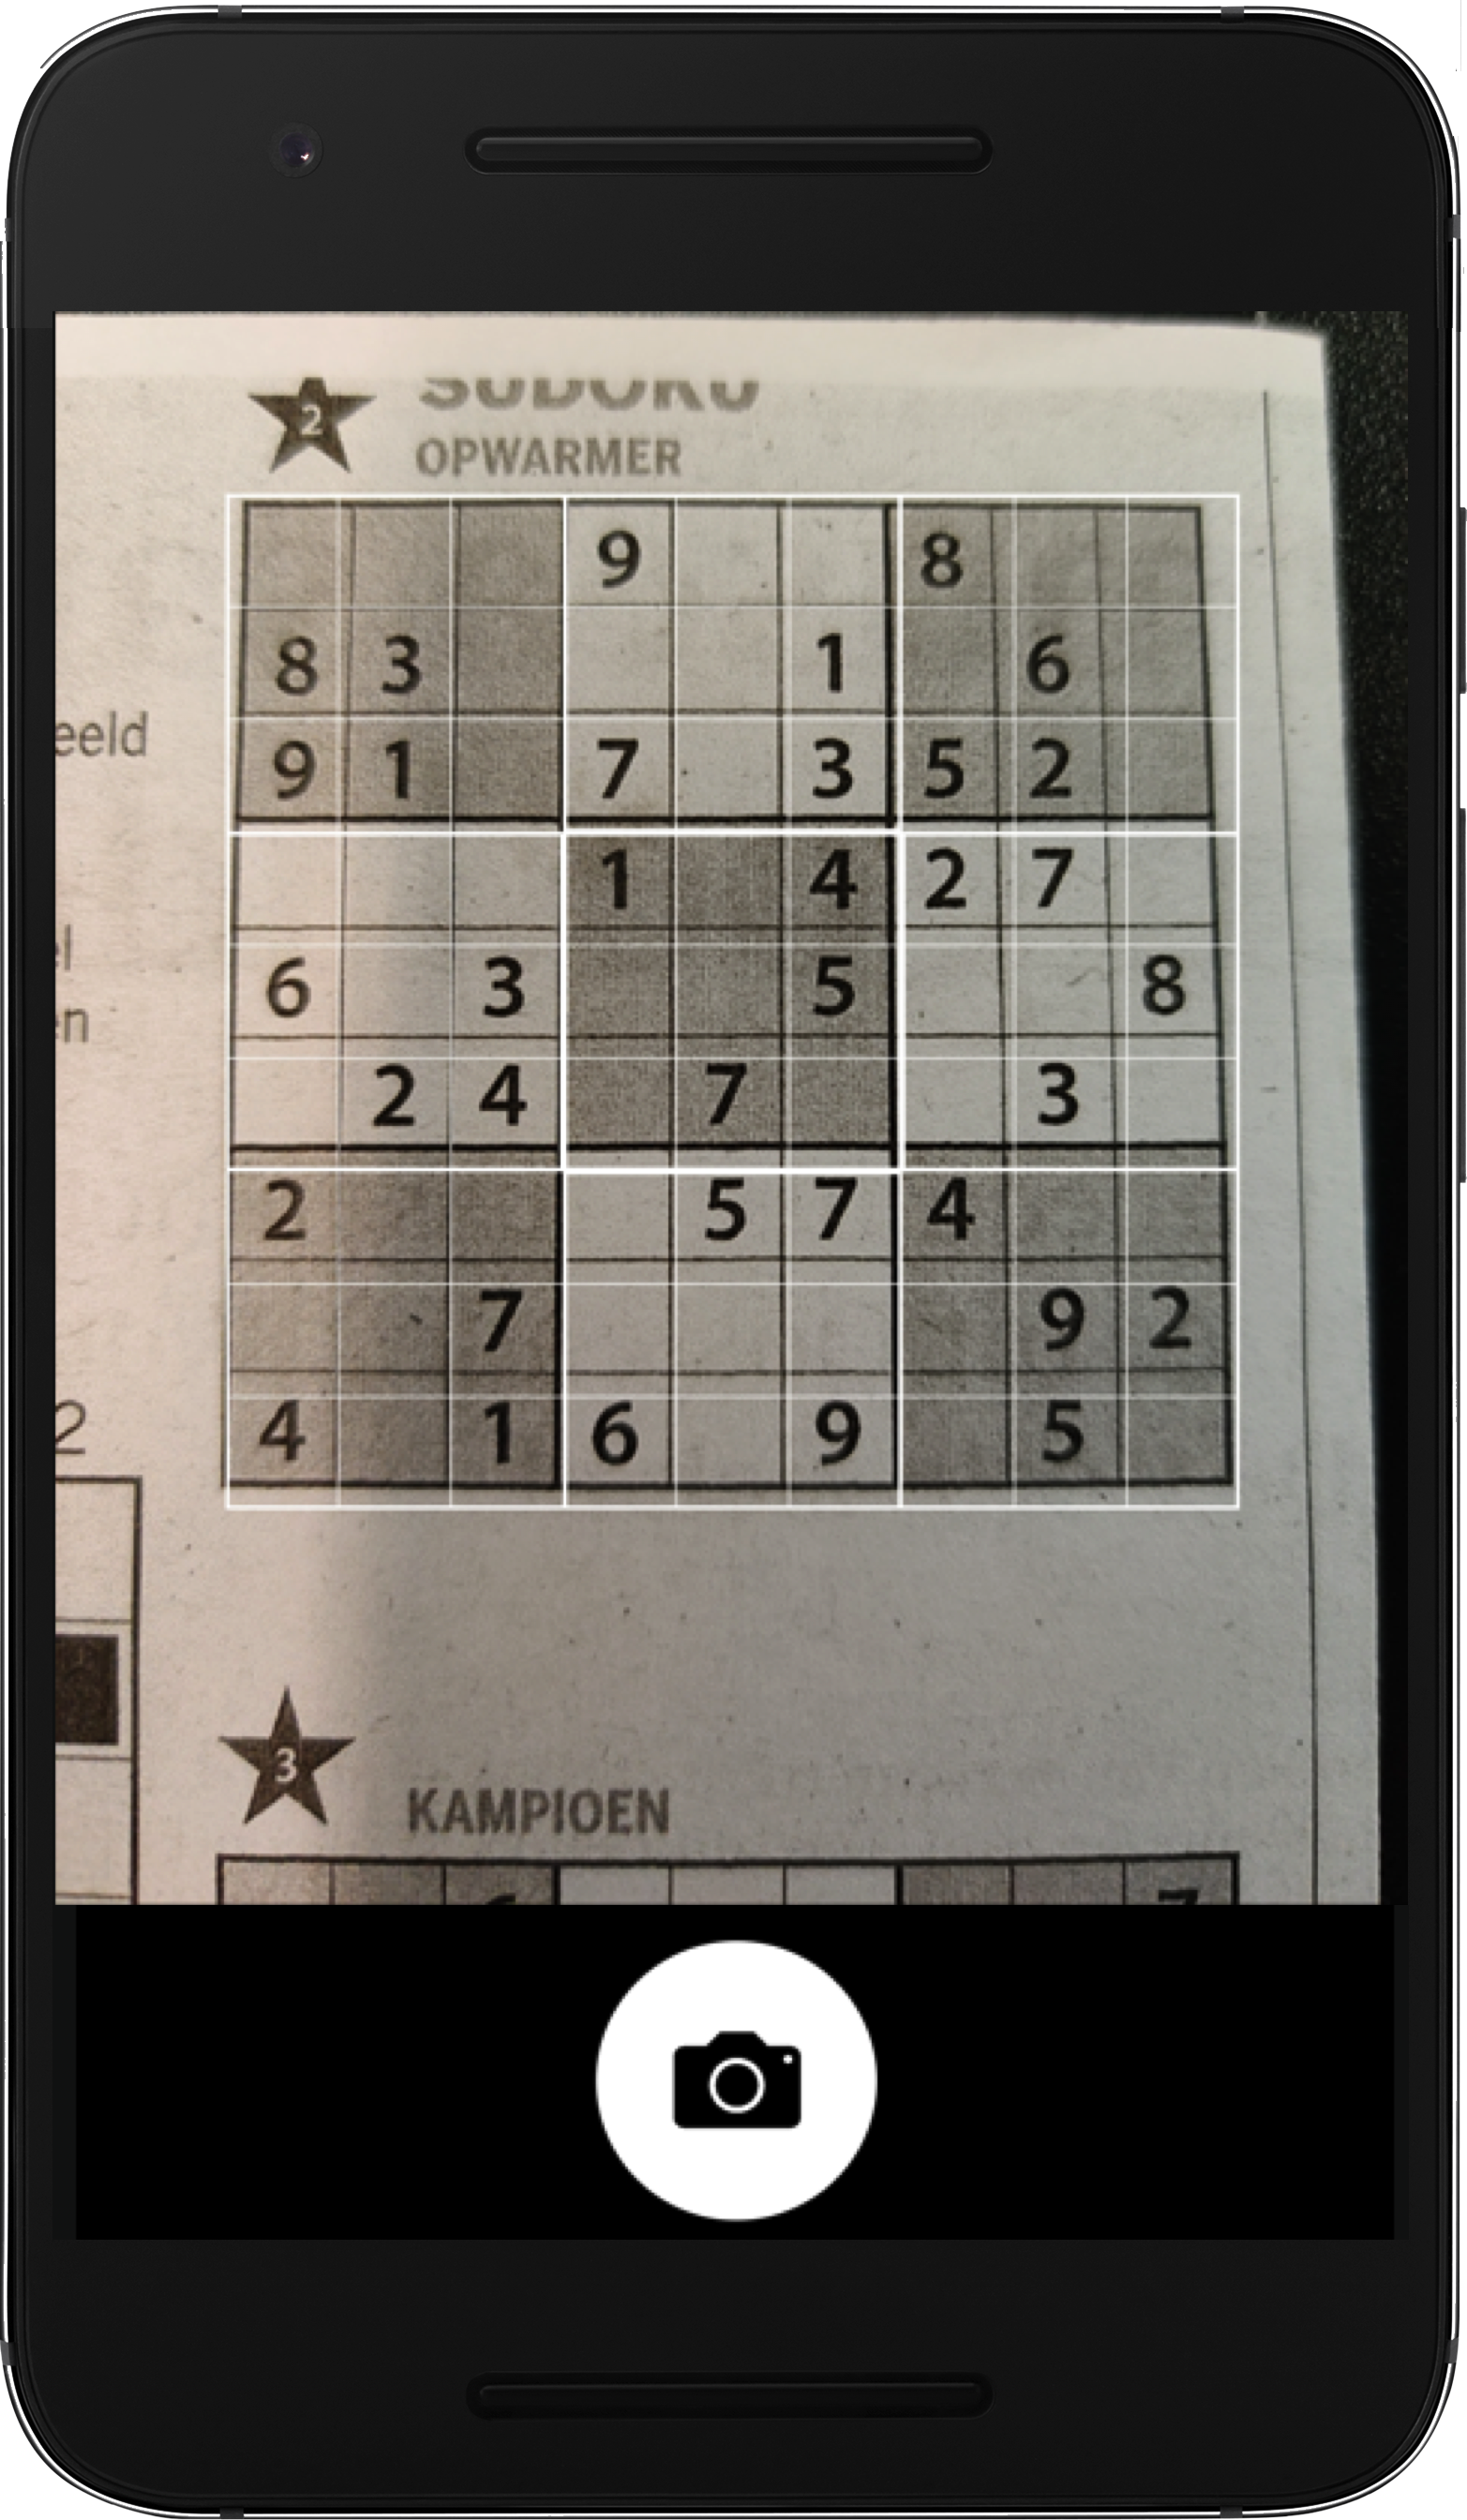
\includegraphics[width=\textwidth]{figures/base_phone-picture.png}
		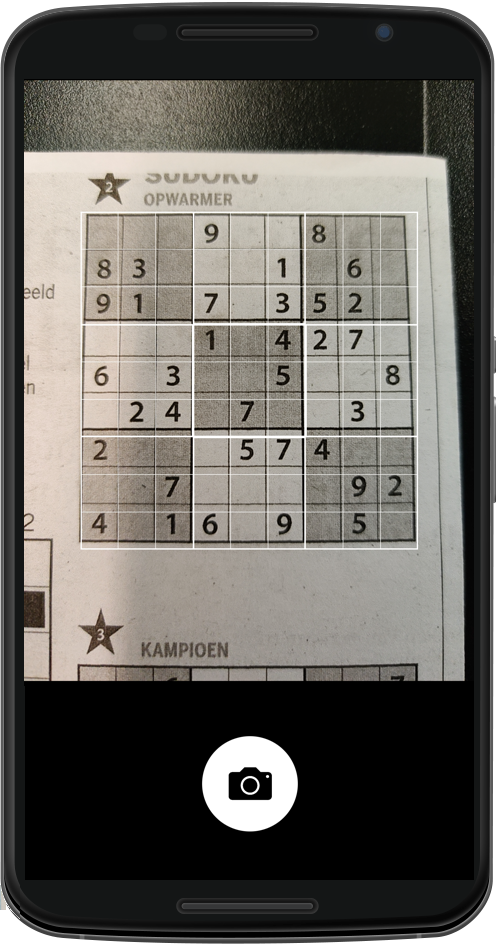
\includegraphics[width=\textwidth]{figures/android-picture.png}	
		\subcaption{}
		\label{fig:camera}
	\end{subfigure}\hfill
	\begin{subfigure}{0.15\textwidth}
		\centering
%		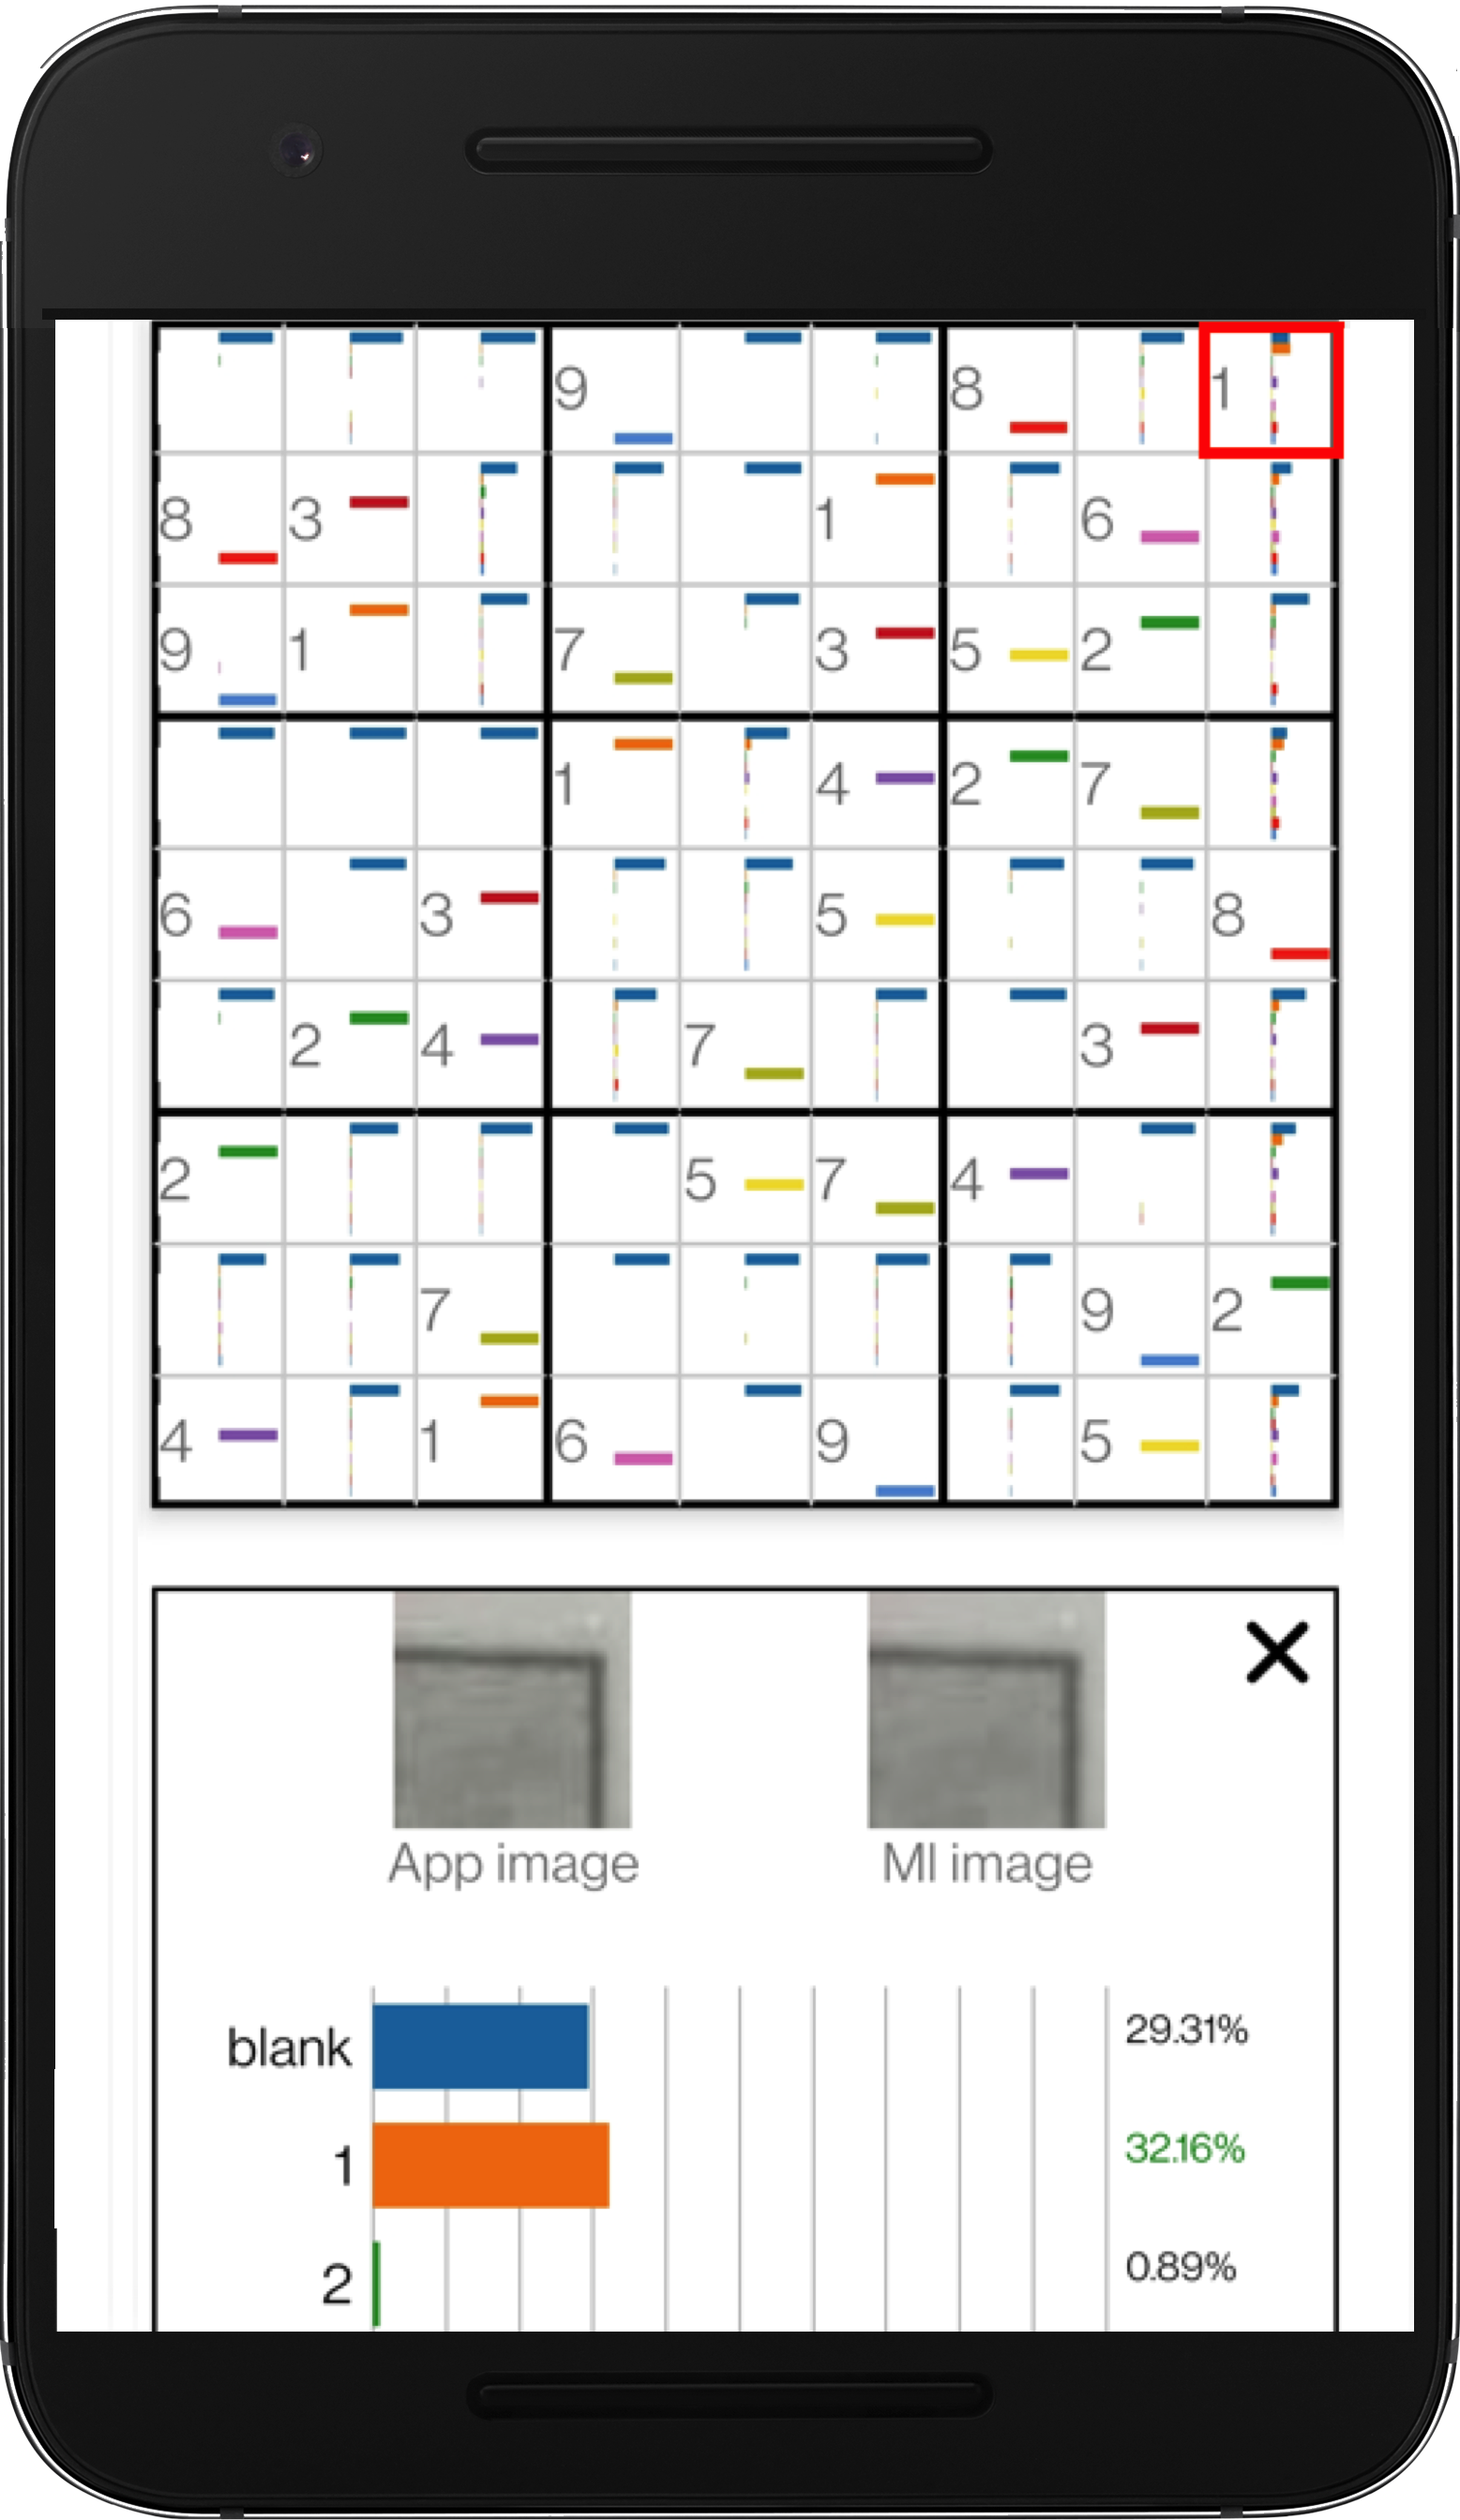
\includegraphics[width=\textwidth]{figures/base_phone-classification.png}
		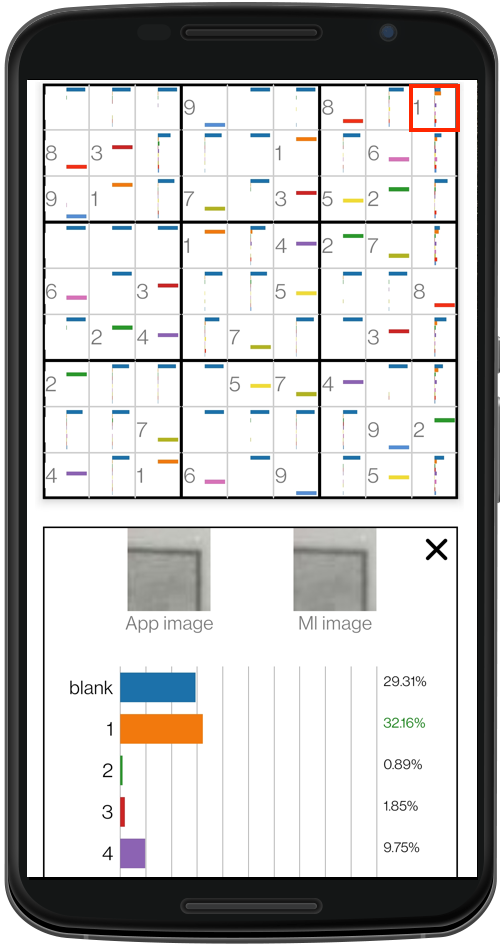
\includegraphics[width=\textwidth]{figures/android-classification.png}
		\subcaption{}
		\label{fig:probas}
	\end{subfigure}\hfill
	\begin{subfigure}{0.15\textwidth}
	\centering
		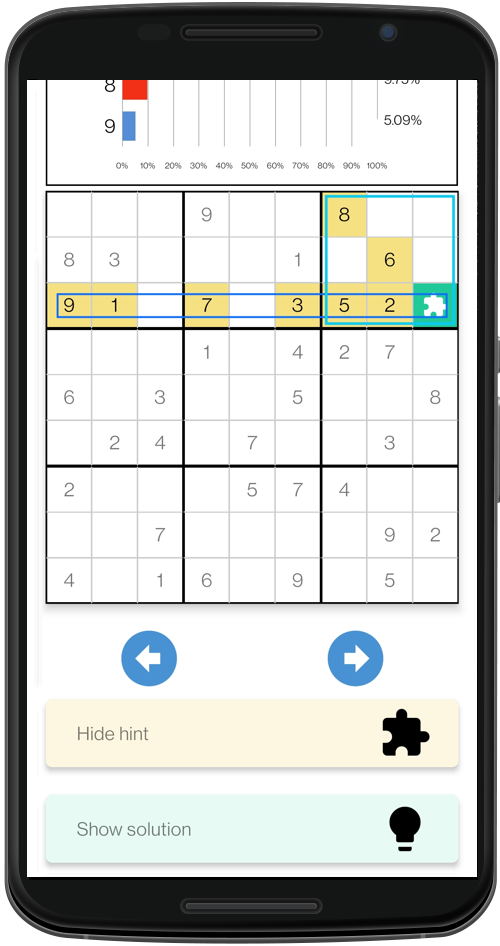
\includegraphics[width=\textwidth]{figures/android-explanation.png}
	\subcaption{}
	\label{fig:explanation}
\end{subfigure}
	\caption{Camera picture of a sudoku (a) with predicted probabilities for the 81 cells (b).Visualisation of the hint (c)
		% where the highlighted constraints and digits can be used to derive a new digit 
		where the highlighted constraints (blue boxes) and given digits (yellow cells) derive a new value at the puzzle piece.
		%(b). Error correction (in red) by the hybrid of prediction and reasoning (c). Visualisation of the hint (d)
		% where the highlighted constraints and digits can be used to derive a new digit 
		%where the highlighted constraints (blue boxes) and given digits (yellow cells) derive a new value at the puzzle piece.
	}
\end{figure}

\begin{figure*}[t]
	\centering
		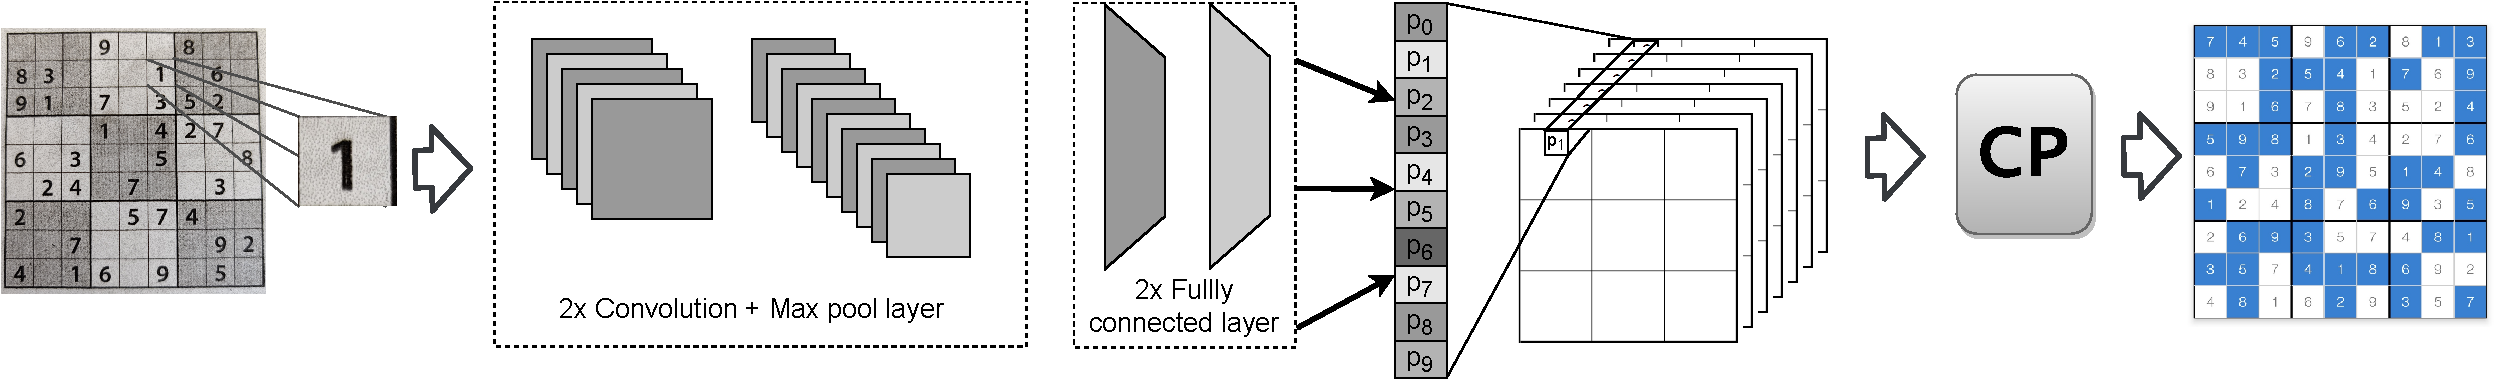
\includegraphics[width=\textwidth]{figures/aaai23-nn_archi.pdf}
%	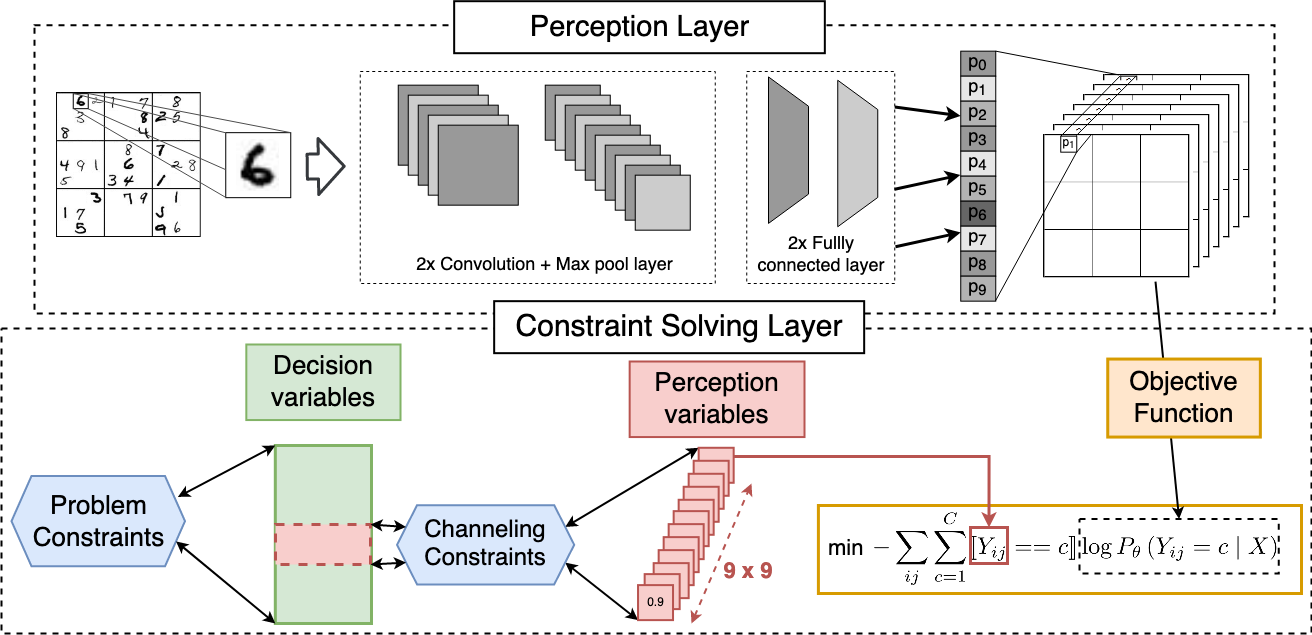
\includegraphics[width=\textwidth]{figures/nn_archi_updated-maxime_diagram.png}
	\caption{The hybrid prediction-and-reasoning approach. }
	\label{fig:hybrid}
\end{figure*}

\paragraph{Classification and Solving}
After the probability distributions have been predicted, a naive approach would simply assign to each cell the value with which the largest probability has been associated (i.e., the argmax). This partial Sudoku can then be given to a constrained satisfaction (CSP) solver, together with the puzzle constraints, to obtain the full solution. However, consider that with this approach, even a CNN with an accuracy of $99\%$ would lead to a correct solution only approximately $0.99^{81} = 44\%$ of the time. This is the case because even a single misclassification almost always leads to a wrong solution or no solution at all.

\paragraph{Better predictions with a hybrid of prediction and reasoning}
Therefore, we proposed an alternative approach in \cite{mulamba2020hybrid}, which features a deeper integration of the digit classification and the reasoning required to solve the Sudoku puzzle. This approach is schematically shown in Fig.\ref{fig:hybrid}. The main idea is to not provide the constraint solver with merely the argmax prediction for each of the Sudoku’s cells, but rather with the full distributions outputted by the CNN. It is then tasked to find the maximum likelihood solution that satisfies the Sudoku constraints, given the class probabilities. Thus, the solver now solves a constrained optimization problem (COP), rather than a CSP. 

In other words, our approach performs a form of joint inference, taking into account the constraints of the Sudoku problem.
Effectively, our hybrid approach allows the reasoning to correct some of the mistakes made by the CNN classifier. 
This allows it to solve significantly more Sudoku problems correctly compared to the naive approach.

\subsection{Phase 2: Human-understandable explanations}
 We want the AI assistant to do more than just show the solution and ruin all the fun for the user. Instead, we want the AI to guide the user into finding the solution, to make them learn some solving strategies along the way.
For this, we integrated explanations from \cite{stepwiseExplaining,OCUS}. 

\paragraph{Providing hints} %A user might be stuck during the solving when faced with a challenging Sudoku. 
The Sudoku Assistant showcases a hinting mechanism that provides the \emph{easiest} next move among all empty cells. 
The provided hint, visualised in Fig. \ref{fig:explanation}, highlights which existing digits and constraints can be used to derive that cell's value. 
The underlying technology relies on a constraint solver to find an Optimal Constrained Unsatisfiable Subset (OCUS) of a derived unsatisfiable formula for (the negation of) each of the empty cells \cite{stepwiseExplaining,OCUS}. 

\paragraph{Explanation difficulty}
%The difference between simple and hard explanations is captured by a cost function that expresses an explanation’s difficulty.
To make sure the provided hints are easy to understand, we rely on a cost function that should approximate human understandability, e.g., taking the number of constraints and digits into account, as well as an estimate of their cognitive complexity.

%In this app, the cost of an explanation is simply the number of constraints involved in it. This reflects the intuition that explanation steps involving many constraints are more difficult to understand than steps with less constraints. 

%To make sure the provided hints are easy to understand, we rely on a cost function that should approximate human understandability, e.g., taking the number of constraints and digits into account, as well as an estimate of their cognitive complexity.

\paragraph{Scalability} 
%% Too slow, therefore we use the ....
Preliminary experiments have shown that generating hints with the out-of-the-box OCUS-algorithm of \citet{OCUS} is too slow for an interactive setting. 
Therefore, we adopt a two-stage approach which works as follows. 
The first stage computes an optimal subset of the problem constraints that can be used to derive a new cell value. 
The second stage first filters the digits of the Sudoku grid that are present in the constraints of the first stage. Next, the system computes the optimal subset of digits required to infer the new cell's value.


%\begin{figure}[!ht]
%	\begin{subfigure}{0.22\textwidth}
%		\centering
%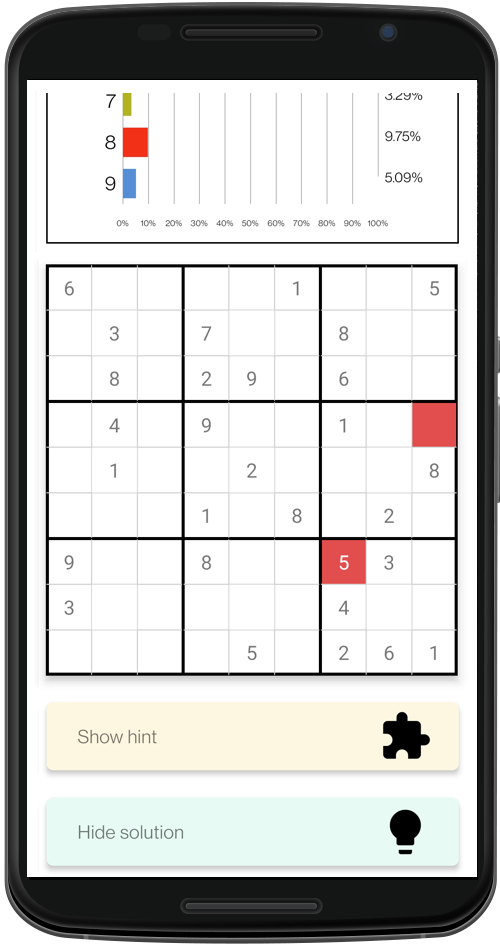
\includegraphics[width=0.7\textwidth]{figures/android-solved.png}
%		\subcaption{}
%	\end{subfigure}\hfill
%	\begin{subfigure}{0.22\textwidth}
%		\centering
%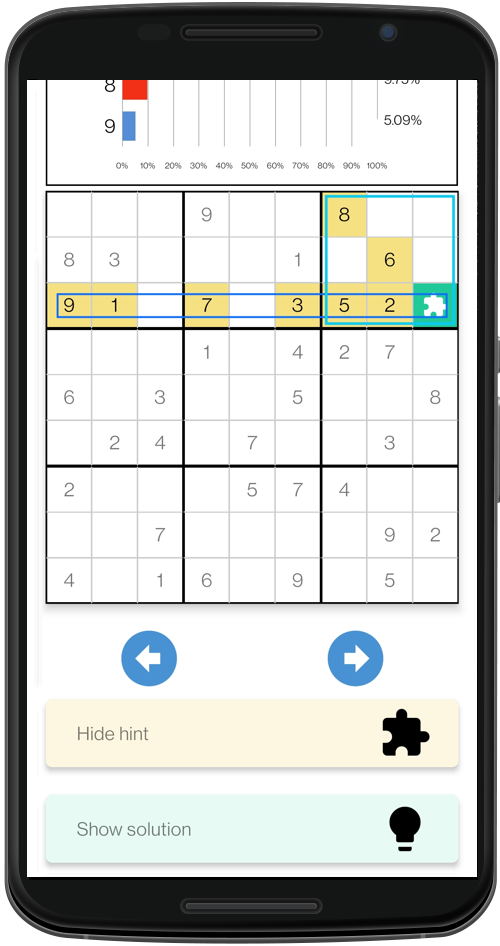
\includegraphics[width=0.7\textwidth]{figures/android-explanation.png}
%		\subcaption{}
%	\end{subfigure}
%	\caption{Error correction (in red) by the hybrid of prediction and reasoning (a). 
%	}
%\end{figure}

%\begin{figure*}[h]
%\begin{subfigure}{0.24\textwidth}
%    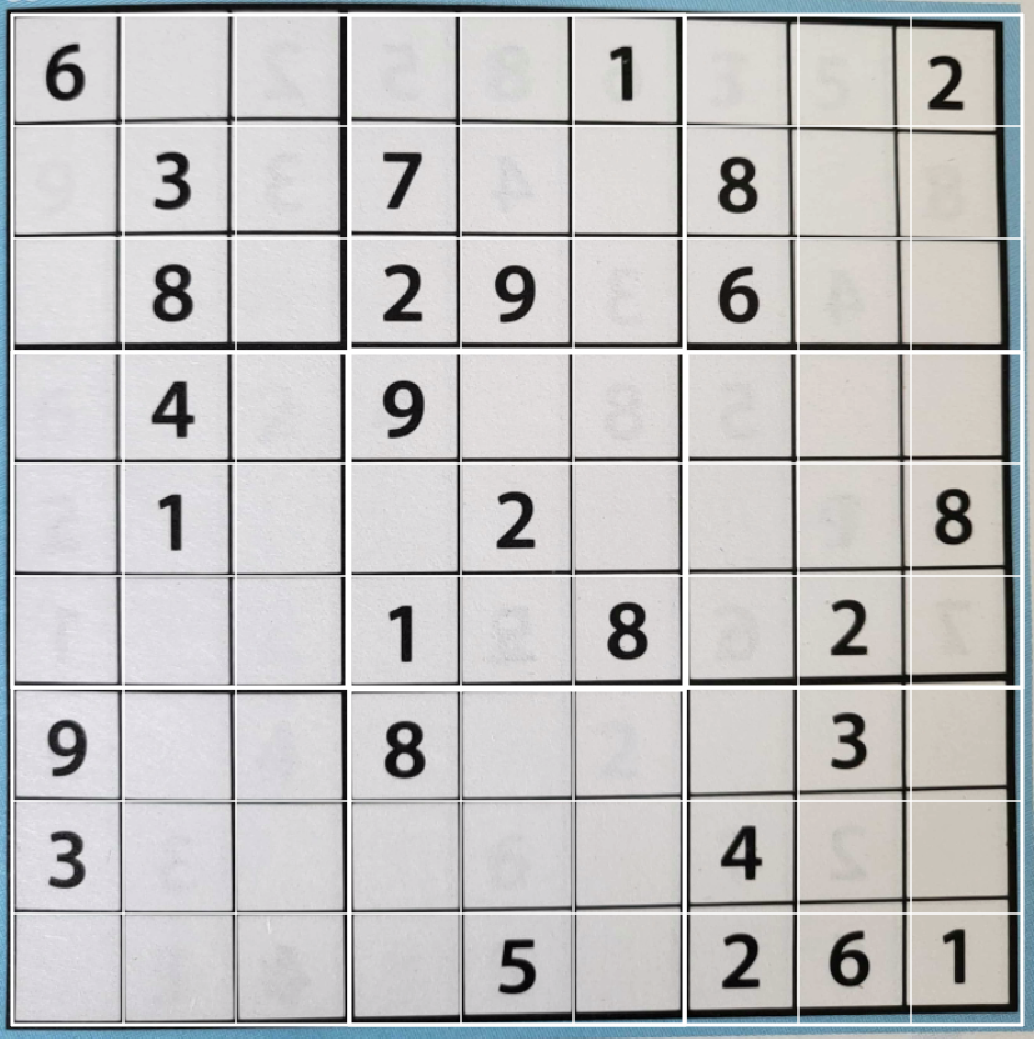
\includegraphics[width=0.99\textwidth]{figures/phone_camera_portrait.png}
%    \subcaption{}
%\end{subfigure}
%\begin{subfigure}{0.24\textwidth}
%    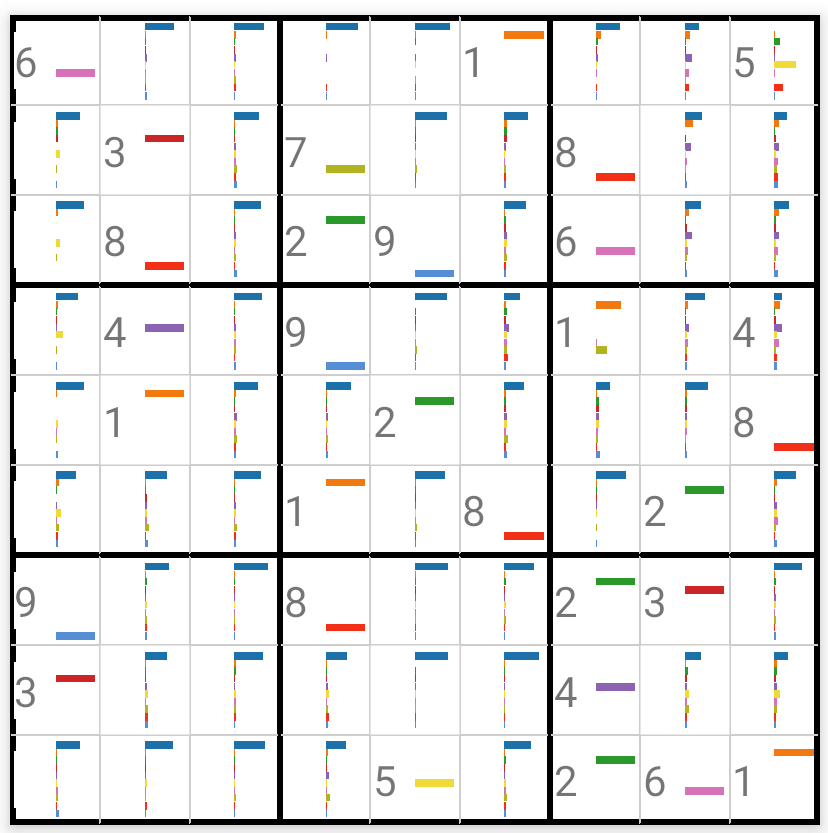
\includegraphics[width=\textwidth]{figures/predictions.png}
%    \subcaption{}
%\end{subfigure}
%\begin{subfigure}{0.24\textwidth}
%    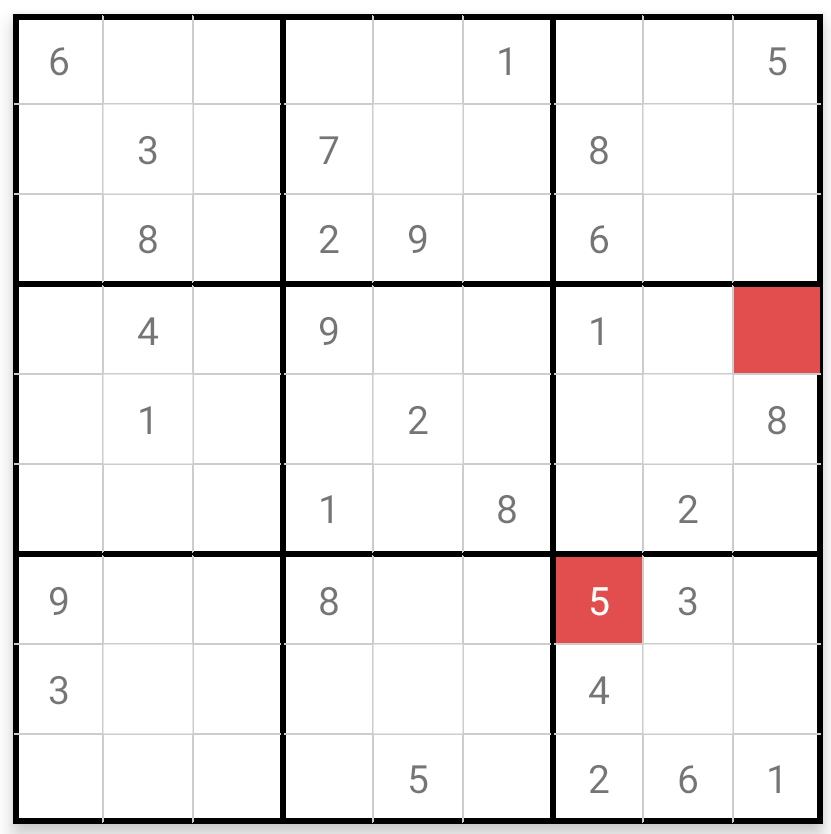
\includegraphics[width=\textwidth]{figures/fix_mistake.png}
%    \subcaption{}
%\end{subfigure}
%\begin{subfigure}{0.24\textwidth}
%    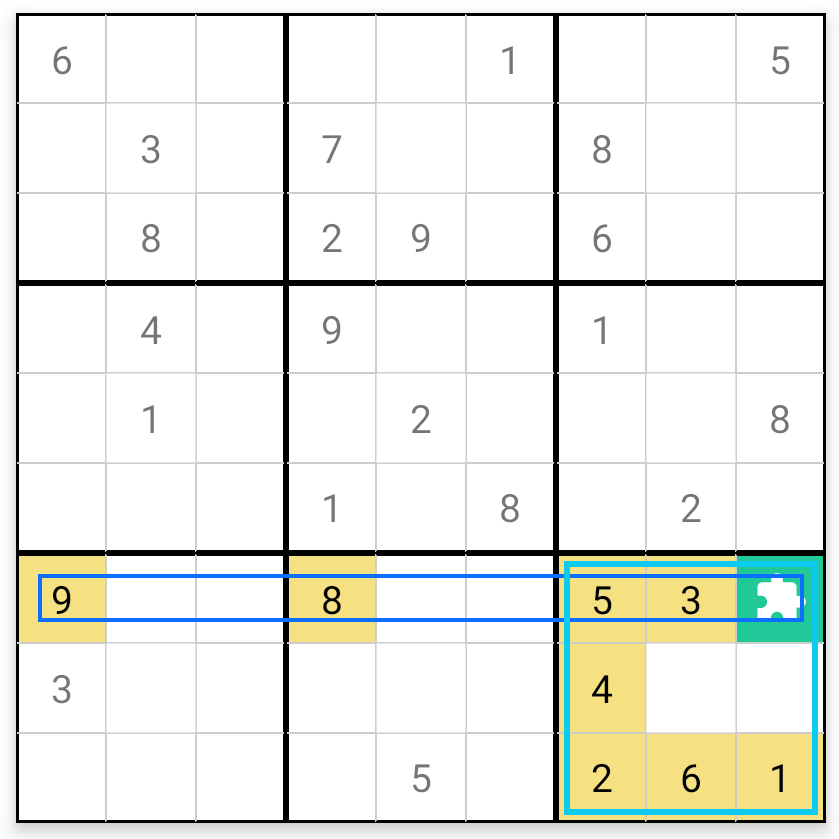
\includegraphics[width=\textwidth]{figures/hint.png}
%    \subcaption{}
%\end{subfigure}
%\caption{Camera picture of a sudoku (a) with predicted probaiblities for the 81 cells (b). Error correction (in red) by the hybrid of prediction and reasoning (c). Visualisation of the hint (d)
%% where the highlighted constraints and digits can be used to derive a new digit 
%where the highlighted constraints (blue boxes) and given digits (yellow cells) derive a new value at the puzzle piece.
%}
%\end{figure*}


\section{Implementation} 
%When solving a Sudoku puzzle, a user might be faced with a contradiction. For instance, same numbers appear in the same column, row, or block. This situation is the direct consequence of an error in the puzzle solving process. 
The app is implemented in React-Native\footnote{Picture of the smartphone is taken from \url{https://toppng.com/android-phone-frame-hd-PNG-free-PNG-Images_78481}}\footnote{Companion website \url{https://visualsudoku.cs.kuleuven.be}}. All neural network and constraint solving computations are done using API calls to a remote server with FastApi. 
The CNN is composed of a VGG-inspired network \cite{VGG}, pre-trained on the Street View House Numbers dataset \cite{SVHN}. 
% EMILIO: Sentence can be removed. If you take it as is, I don't think i5's necessary to say more.} 
 % it is not further trained, this network operates as a backbone that extracts features from the image. 
The last layer is replaced by a two-layers fully-connected neural network, tuned for our classification task using labeled data acquired from the app. All neural networks are implemented with PyTorch 1.10 \cite{pytorch}. All reasoning (the hybrid reasoning and explanation generation) is implemented in the CPMpy 0.9.9 constraint solving environment \cite{cpmpy}.

%The app is available on the google play store at ????? .
%\section{Demonstration}

\section{Related works}
In recent years, the combination of deep learning for image perception and symbolic reasoning to visual sudoku has become increasingly popular.
Some systems jointly learn the constraints to classify cell values~\cite{Pushing, SATNet, NeurASP}. 
However this requires solver-specific mechanisms whereas our approach works with any constraint  solver. 
Another limitation, also present in \cite{CLRD, mulamba2020hybrid} is that instances are built by sampling images from MNIST \cite{mnist}, on which recent machine learning approaches achieve near-perfect accuracy \cite{ensemble-mnist}. Images from a phone camera are in RGB space, can contain artifacts such as grid borders and are overall noisier depending on the angle of the camera or lighting conditions. They are a bigger challenge. 

A non-exhaustive list of works \cite{reeson2007interactive,caine2007tutoring}, showcase (interactive) tutoring systems using the Sudoku puzzle, for instance, to teach consistency propagation algorithms in Constraint Programming \cite{howell2018solving}. 
Other works rely on Minimal Unsatisfiable Subsets (MUS) to compute a minimal subset of constraints and facts that can be used to derive new information \cite{stepwiseExplaining,espasa2021using}. Few works have considered optimizing MUSs with respect to a given cost-function. The only criterion considered is cardinality-minimality \cite{conf/sat/LynceM04,ignatiev2015smallest}.

\section{Conclusion and Future work}

The Sudoku Assistant App combines machine learning and constraint reasoning to interpret, solve and explain pen-and-paper sudokus. 
The system has room for further improvements. As illustrated in Fig. \ref{fig:camera}, the user must align the grid overlay with the target sudoku. 
A potential improvement in the image acquisition is to train a CNN to extract a sudoku from an image, as done in Object Detection~\cite{TableNet}. 

The hint mechanism of the Sudoku Assistant relies on a simplistic cost-function to approximate the cognitive complexity of an explanation.
An open question there is how to design a cost function that better reflects the human-interpretability of explanations. 

Finally, we can assume that printed numbers usually are initial clues of the puzzle, and that hand-written numbers usually are  from human input. The constraint solver could focus more on printed numbers while searching the feasible space. 

%\begin{enumerate}
%    \item How can the cost function be improved to reflect the cognitive complexity of the explanations?
%    \item Recognizing the printed digits from the written digits?
%    \item Auto-take a picture when the sudoku is recognized?
%\end{enumerate}
% 
%


%\begin{figure*}[!ht]
%	\begin{subfigure}{0.24\textwidth}
%		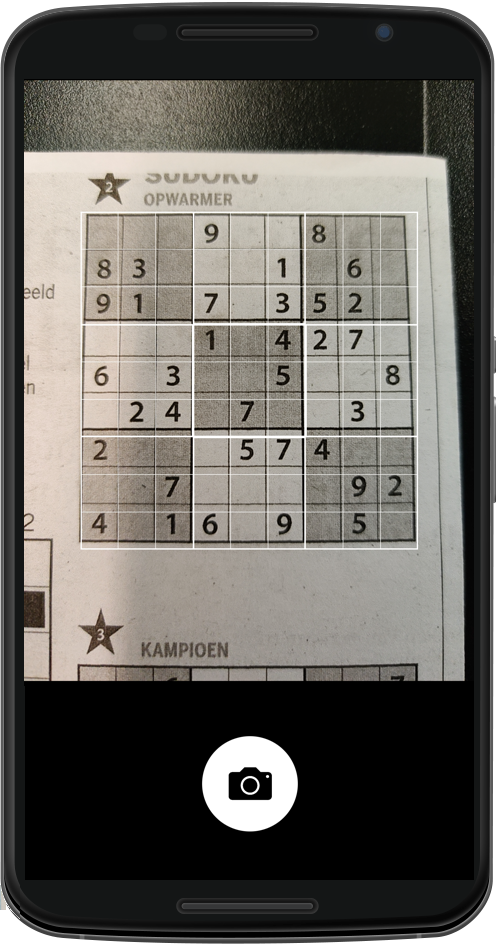
\includegraphics[width=0.99\textwidth]{figures/android-picture.png}
%		\subcaption{}
%	\end{subfigure}
%	\begin{subfigure}{0.24\textwidth}
%		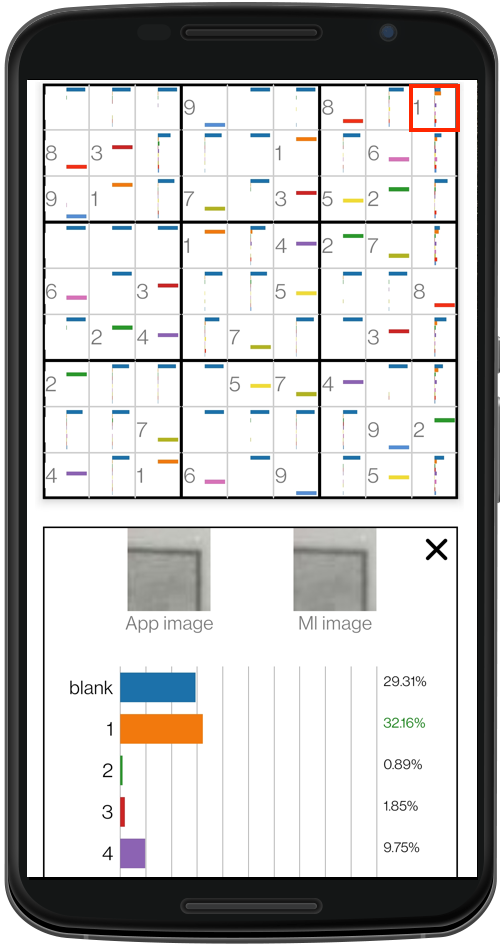
\includegraphics[width=\textwidth]{figures/android-classification.png}
%		\subcaption{}
%	\end{subfigure}
%	\begin{subfigure}{0.24\textwidth}
%		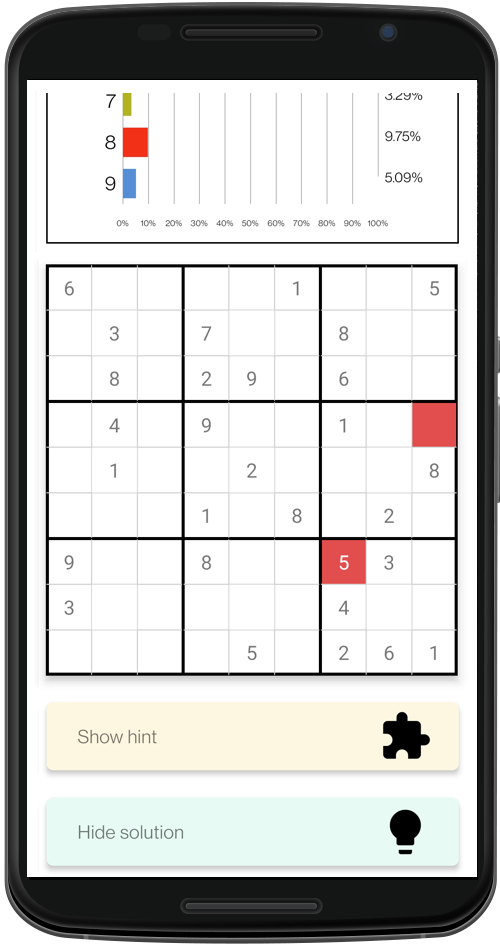
\includegraphics[width=\textwidth]{figures/android-solved.png}
%		\subcaption{}
%	\end{subfigure}
%	\begin{subfigure}{0.24\textwidth}
%		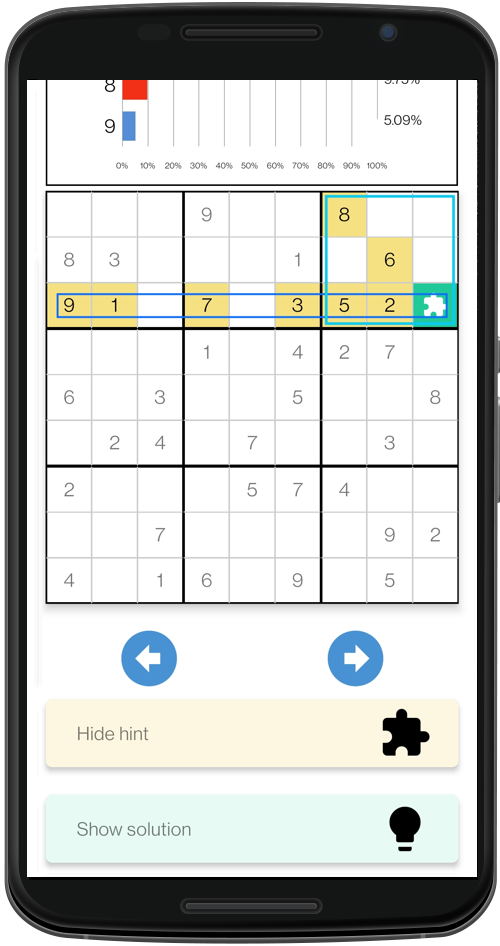
\includegraphics[width=\textwidth]{figures/android-explanation.png}
%		\subcaption{}
%	\end{subfigure}
%	\caption{Camera picture of a sudoku (a) with predicted probaiblities for the 81 cells (b). Error correction (in red) by the hybrid of prediction and reasoning (c). Visualisation of the hint (d)
%		% where the highlighted constraints and digits can be used to derive a new digit 
%		where the highlighted constraints (blue boxes) and given digits (yellow cells) derive a new value at the puzzle piece.
%	}
%\end{figure*}

\clearpage
\section{Acknowledgements}
This research received partial funding from the Flemish Government (AI Research Program); and funding from the European Research Council (ERC) under the European Union’s Horizon 2020 research and innovation program (Grant No. 101002802, CHAT-Opt).


\bibliography{aaai23.bib}  
% \nobibliography{aaai23}


\end{document}
